% % Created 2015-09-15 Tue 11:46
% \documentclass[11pt]{article}
% \usepackage[utf8]{inputenc}
% \usepackage[T1]{fontenc}
% \usepackage{fixltx2e}
% \usepackage{graphicx}
% \usepackage{longtable}
% \usepackage{float}
% \usepackage{wrapfig}
% \usepackage{rotating}
% \usepackage[normalem]{ulem}
% \usepackage{amsmath}
% \usepackage{textcomp}
% \usepackage{marvosym}
% \usepackage{wasysym}
% \usepackage{amssymb}
% \usepackage{hyperref}
% \usepackage{color}
% \usepackage{soul}
% \tolerance=1000
% \usepackage[margin=1in]{geometry}

% \newcommand{\hilight}[1]{\colorbox{yellow}{#1}}

% %\author{Alex Ansari}
% %\date{}
% %\title{TALOS}
% %\hypersetup{
% %  pdfkeywords={},
% %  pdfsubject={},
% %  pdfcreator={Emacs 24.3.1 (Org mode 8.2.10)}}


% \begin{document}
\section{Hydraulic Lower Extremity Exoskeleton}

Exoskeleton suit was originally developed for military uses, specifically to allow operators to perform motions without incurring muscle fatigue.  Their main contributions in the literature re based on a {\bf virtual joint torque control}, which has been shown to be an effective human robot interaction control strategy in situations where the connections between the uses and hardware system are relatively unknown or can dramatically change as a function of time.

Additionally, the hardware system focuses on actuator selection.  The main hardware design principle is focused on developing a suit that can augment a users power and move fast when necessary.  They selected hydraulic actuation because the addition of electric actuator weight on the system leg joints makes the system difficult to move quickly.  On the other hand, hydraulic actuators have high power density relative to weight and size, and generally provide very high force outputs and low impedance.  The tradeoff with hydraulics come in the way of having low accuracy in terms of force control as well as hard to model nonlinear characteristics.  

A picture of the Hydraulic Lower Extremity Exoskeleton is presented in Figure \ref{fig:exoSuit}.
\begin{figure}[thpb]
\centering
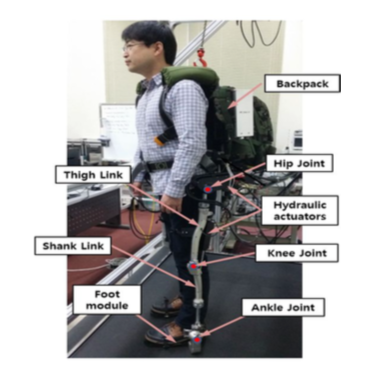
\includegraphics[width=3.in]{exos/figs/hydLowerExrem/exoSuit}
  \caption{}
  \vspace{-0.2in}
 \label{fig:exoSuit}   
 \end{figure} 

\subsection{Actuator specifications}

The actuator specifications for the Hydraulic Lower Extremity Exoskeleton were designed around human walking data at 4km/h with a 45 kg load.  The resulting calculated hydraulic capacity for the while system was 2050psi and 8lpm.  The individual actuators were designed to be double acting at the hip and knee flexion/extension joints. The {\bf hip maximum thrust was 4 kN} and {\bf knee maximum thrust was 4 kN}.  Each joint joint included three-way servo valves (M 200, Star-Hydraulic) to control rate and direction of bi-directionality and bypass valves to connect the pump path to tank path for fast, energy efficient motion during swing phases.   

The hydraulic system for each joint is shown in Figure \ref{fig:hydraulicSys}.
A picture of the Hydraulic Lower Extremity Exoskeleton is presented in Figure \ref{fig:exoSuit}.
\begin{figure}[thpb]
\centering
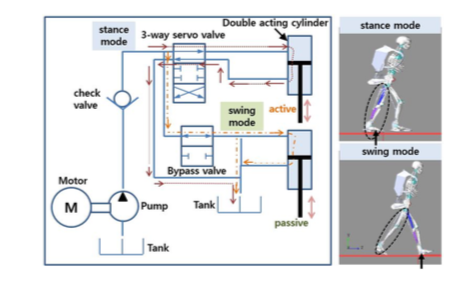
\includegraphics[width=3.in]{exos/figs/hydLowerExrem/hydraulicSys}
  \caption{}
  \vspace{-0.2in}
 \label{fig:hydraulicSys}   
 \end{figure} 


%\begin{figure}[thpb]
%\centering
%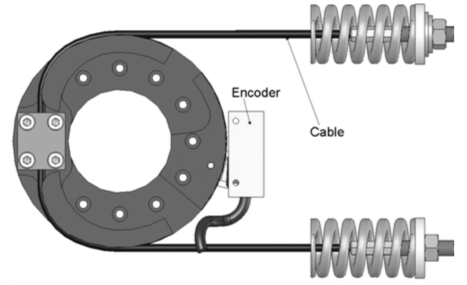
\includegraphics[width=3.in]{figs/seaAssm}
%  \caption{}
%  \vspace{-0.2in}
% \label{fig:IHMCSEA}   
% \end{figure}
 

 
 \subsection{Exoskeleton Specifications}
 
 The Hydraulic Lower Extremity Exoskeleton includes four actively controlled joints in the sagittal plane; the knee and hip flexion/extension degrees of freedom are powered degrees of freedom for each leg.  The hardware also includes eight passive joints: one ab/adduction DOF for each hip and three degrees of freedom for each ankle.
 
 The hydraulic system of the suit is composed of the four actuators and a hydraulic power unit, consisting of a pump, motor, temperature sensor, and various valves.
 
 Additionally, various {\bf sensors} are incorporated to measure joint angles, actuator forces , and ground reaction forces.  Three absolute angular encodes are incorporated at the hip, knee, and ankle pitch joints.  In-line load cells are incorporated in each cylinder tube to measure actuator forces, and four single axis load cells are included in foot sensors to be used for gait phase detection.
 
 \subsection{Control Specifications}
 
 \begin{figure}[thpb]
\centering
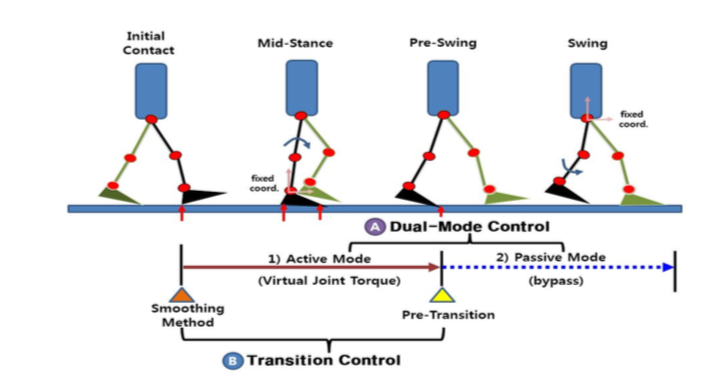
\includegraphics[width=5.in]{exos/figs/hydLowerExrem/dualModeDia}
  \caption{}
  \vspace{-0.2in}
 \label{fig:dualModeDia}   
 \end{figure}
The control design principle for the Hydraulic Lower Extremity Exoskeleton is base around the concept that, for walking gaits, the {\bf stance and swing controllers should be considered separately}.  To this end, the literature for this hardware system introduces an active-passive control method called {\bf Dual-Mode Control}.  Active control is used during stance phases whereas the passive control is used to quickly and freely control the system's legs during swing phases.  Additionally, to handle the inherently discontinuous jumps in the command signals that occur as a function of this dual mode abstraction, a smoothing method is introduced that is used in conjunction with a pre-transition method that solves the swing delay due to internal cylinder pressure.  A diagram which highlights the different modes in this control strategy is shown in Figure \ref{fig:dualModeDia}.   

Various components of the overall dual-mode control strategy, at the hardware level, are presented in Figure \ref{fig:suitDia}.  
  \begin{figure}[thpb]
\centering
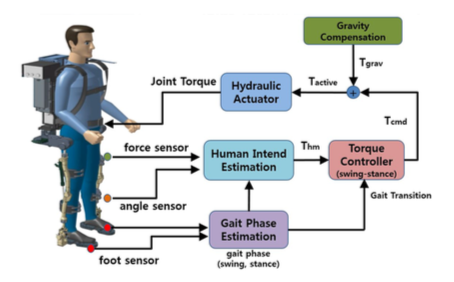
\includegraphics[width=3.in]{exos/figs/hydLowerExrem/suitDia}
  \caption{}
  \vspace{-0.2in}
 \label{fig:suitDia}   
 \end{figure}
This figure contains a number of components, specifically a {\bf gait phase estimation block} which uses the foot sensors to estimate the stance mode of the system, a {\bf human intention block}, which uses angular encoders and joint force sensors to estimate the motion of the operator, a {\bf torque controller}, and a {\bf gravity compensation} block.  Note that these various components of the control system are used to support the general assumption of the dual mode controller, i.e., 
 \begin{figure}[thpb]
\centering
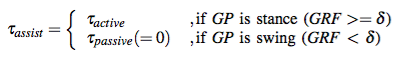
\includegraphics[width=3.in]{exos/figs/hydLowerExrem/torAssist}
  \caption{}
  \vspace{-0.2in}
% \label{fig:suitDia}   
 \end{figure}
 
 \noindent
where, $GP$ is the gait phase, $GRF$ is the ground reaction force, and $\delta$ is a threshold value.  This equation explicitly states that an active torque will be applied for each leg during stance and that the legs are passive in their respective swing phases.

Like other control methods presented in this report, the dual mode control method in this section uses the fundamental assumption that it is difficult to measure the interaction forces between the user and hardware system directly as a primary design principle.  To this end, the human-robot interaction force is assumed to be completely represented in terms of the joint torque applied by the operator in the hardware. 

To calculate the active torque applied to the joints during the active mode control, the robot dynamics are considered independently from the operator, namely,
\begin{equation}
T_a = M(q)\ddot{q} + C(q,\dot{q})\dot{q}+G(g),
\label{dynamics}
\end{equation}   
where $T_a$ is the joint torque applied by the actuators, $M(q)$ is the inertia matrix, $C(q,\dot{q})$ is the centripetal and Coriolis matrix, and $G(q)$ is the gravitational torques. note that this equation neglects friction as well as other actuation dynamics.

Using the force sensors on the hydraulic actuators, the {\bf human-robot interaction torques} can be approximated as
\begin{equation}
\hat{T}_{hm} = M_n(q)\ddot{q} + C_n(q,\dot{q})\dot{q} + G_n(q) - \hat{T}_a, \notag
\end{equation}
where $M_n$, $C_n$, and $G_n$ are the nominal models of the true inertia, centripetal, and gravitational parameters and $\hat{T}_a$ represents the measured actuator torques.  The $M_n(q)\ddot{q} + C_n(q,\dot{q})\dot{q} + G_n(q) $ portion of $\hat{T}_{hr}$ represents the inverse dynamics component of the closed-loop control system.  The overall joint torque controller, which combines compensation to for operator intent as well as balancing the suit under a gravitational load is then written \[ \tau_\text{active} = K(s) \hat{T}_{hm} + G_n(q),\] where $K(s) = K_p +s K_d,$ i.e., there is closed-loop PD control law operating on the error between the predicted robot dynamics and the measured joint torques.  The block diagram for the active mode controller is shown in Figure \ref{fig:blockDia}. 
 \begin{figure}[thpb]
\centering
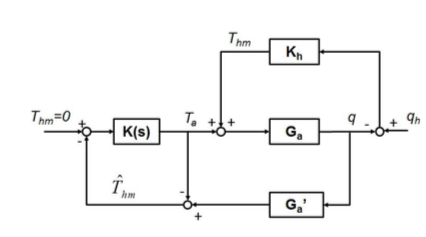
\includegraphics[width=3.in]{exos/figs/hydLowerExrem/blockDia}
  \caption{}
  \vspace{-0.2in}
 \label{fig:blockDia}   
 \end{figure}
 Note that $G_a$ represents the dynamics of the the system and $G_a'$ the inverse dynamics model in Figure \ref{fig:blockDia}.

In the passive mode, which occurs during the swing phase, the leg of the human-robot system moves quickly and freely under using the passive inertial forces of the overall system.  This is accomplished using bypass valves that connect the pump path to the tank path to achieve mechanical back-drivability.  The foot sensors on each foot are used to trigger the bypass valves and to initiate the pass control mode.

A novel component in the literature of the Hydraulic Lower Extremity Exoskeleton controller is how the transitions between the active and passive control modes are handled.  In particular, an explicit smoothing method is used to address the discontinuity in the command torque at phase transitions.  One solution which is proposed is to use an exponential weighting function of the form
 \begin{figure}[thpb]
\centering
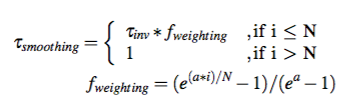
\includegraphics[width=3.in]{exos/figs/hydLowerExrem/weightingForm}
  \caption{}
%  \vspace{-0.2in}
% \label{fig:suitDia}   
 \end{figure}
 
 \noindent
 where $\tau_\text{inv}$ is the inverse dynamics torque associated with the robot model, $f_\text{weighting}$ is the weighting function, $a$ is a sensitivity factor, and $N$ describes the duration of the transition period.  The transition duration period as well as sensitivity factor appear to be hand tuned parameters. 

In addition to phase transition smoothing a pre-transition control method which happens at the end of the stance phase prior to the passive swing phase is also used to effect smooth phase transitioning.  The pre-transition control works by measuring the ground reaction force and setting a minimum threshold value.  When the GRF drops below the threshold, the passive swing control mode is entered, i.e., the bypass valve at the actuators are opened.  The objective of this method is to reduce the phase transition delay due to residual pressure in the foot sensors. 


 
 \subsection{Opinion}
 
The design of the Hydraulic Lower Extremity Exoskeleton has a lot going for it.  The best part of this hardware as well as control design is the fact that the creators of it are doing something relatively straightforward.  The actuators are composed of what appears to be off-the-shelf components, and the addition of bypass valves to take advantage of passive dynamics during walking to produce more energy conscious behaviors is a good idea.    

One potential drawback of this hardware is the power system.  The documentation in \cite{} was sparse with respect to the exact specifications of the motor and energy storage device which powers the hydraulic system.

The control system for this hardware followed a relatively straight-forward design, effectively creating a ``get out of the way design" using the torque sensed at the joints only.  In the short-term, this type of policy seems to be a good strategy.  The other highlight of the outlined control policy was the smoothing function which was used during phase transitions in the walking gait cycle.  A similar type of smoothing will most likely be beneficial in terms of operator experience for a varity of different operational modes in which different phase transitions occur, e.g., running, jumping, etc.
 
 
 % \end{document}

 
 % Hongchul Kim and Changhoon Seo and Young June Shin and Jung Kim and Youn Sik Kang, "Locomotion Control Strategy of Hydraulic Lower Extremity Exoskeleton Robot," IEEE International Conference on Advanced Intelligent Mechatronics, 2015, pp. 577-582.
 
 
 